%%%% Weekly Report Information %%%%
\newcommand{\handoutName}{Weekly report}
\newcommand{\handoutdate}{Nov 18, 2014}
\newcommand{\duedate}{}
% Header template used for Weekly Reports
\documentclass[11pt,twoside]{article}

\setlength{\oddsidemargin}{0pt}
\setlength{\evensidemargin}{0pt}
\setlength{\textwidth}{6.5in}
\setlength{\topmargin}{0in}
\setlength{\textheight}{8.5in}
\setlength{\voffset}{0in}

\providecommand{\titlesize}{small}


\usepackage{graphicx}
%\usepackage{subfigure}
\usepackage{palatino}
%\usepackage{cmbright}
\newcommand{\myMargin}{1.00in}
%\usepackage[pdftex]{hyperref}
\usepackage[small,bf]{caption}
\usepackage{amsmath}
\usepackage[usenames,dvipsnames]{color}
\usepackage{fancyhdr}
\pagestyle{fancy}
\usepackage{datetime}
\usepackage{fancyvrb}
\usepackage{color}
\usepackage[\titlesize, compact]{titlesec}
\usepackage{multicol}
\usepackage{enumitem}
\usepackage{pdfpages}
\usepackage{mdwlist}


\usepackage[ruled]{algorithm}
\usepackage{algpseudocode}

\usepackage{caption}
\usepackage{subcaption}



\newdateformat{dashdate}{\THEYEAR-\twodigit{\THEMONTH}-\twodigit{\THEDAY}}
\def\Tiny{\fontsize{3pt}{3pt}\selectfont}

\providecommand{\handoutName}{Handout title}
\providecommand{\handoutdate}{Handout date}
\providecommand{\duedate}{}

\lhead{Meeting with Prof. Becker\\
Fall, 2014}
\chead{}
\rhead{ Shiva Shahrokhi\\
\handoutdate }
\lfoot{}
\cfoot{\thepage}
\rfoot{\dashdate \Tiny \textcolor{Gray}{\today}}
\renewcommand{\headrulewidth}{0.4pt}
\renewcommand{\footrulewidth}{0.4pt}

\begin{document}

\vspace{0.60in}
\begin{center}
{\Large\textbf{\handoutName}}\\
\vspace{0.03in}
\textbf{\duedate}\\
\end{center}

\newcommand{\todo}[1]{
  \textcolor{Red}{
    \begin{tabular}{|c|}
      \hline
      \em \large \bfseries todo: \normalfont \normalsize #1 \\
      \hline
    \end{tabular}}
}


\section{My \emph{Objectives} this week}
\begin{itemize}
\item Showing mean position in code.
\item Plotting different gain values and finding the best
\item varying noise and see the influence.
\item 2D control position
\item What is better to control? Variance or standard deviation?
\end{itemize}


\section{My \emph{Accomplishments} this week}

\subsection{\emph{Auto Controllers}}

\begin{itemize}
\item different gain values.
\end{itemize}

\begin{figure}[!htb]
\captionsetup{justification=centering}
\minipage{0.32\textwidth}
  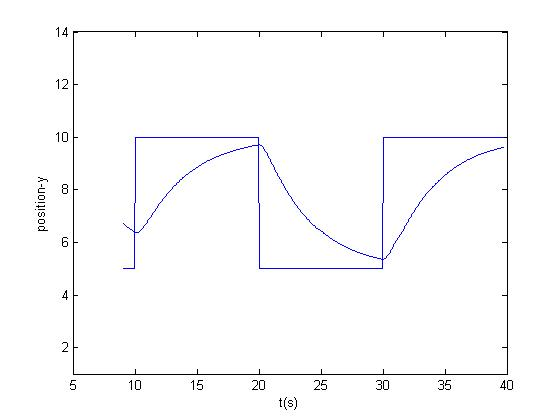
\includegraphics[width=\linewidth]{fig/gain1d1.jpg}
  \caption{kgain 1 and derivative 1}
\endminipage\hfill
\minipage{0.32\textwidth}
  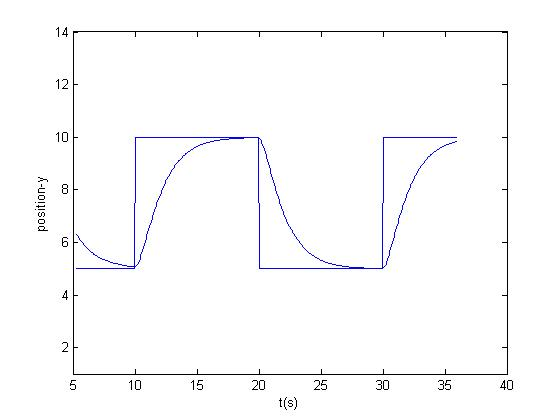
\includegraphics[width=\linewidth]{fig/gain2d1.jpg}
  \caption{kgain 2 and derivative 1}
\endminipage\hfill
\minipage{0.32\textwidth}%
  %\includegraphics[width=\linewidth]{shiva444.eps}
  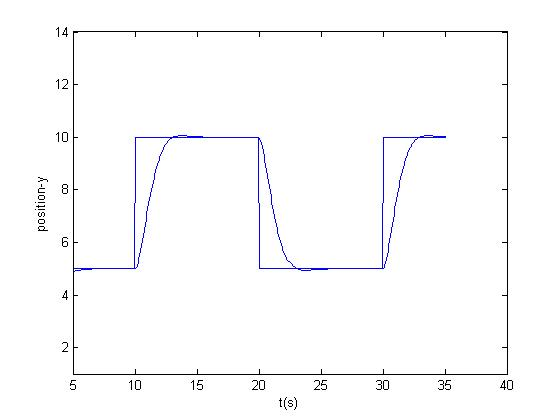
\includegraphics[width=\linewidth]{fig/gain4d1.jpg}
  \caption{kgain 4 and derivative 1}
\endminipage
\end{figure}
\begin{figure}[!htb]
\captionsetup{justification=centering}
\minipage{0.32\textwidth}
  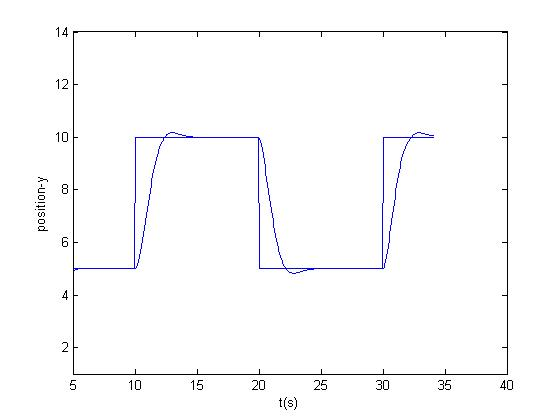
\includegraphics[width=\linewidth]{fig/gain5d1.jpg}
  \caption{kgain 5 and derivative 1}
\endminipage\hfill
\minipage{0.32\textwidth}
  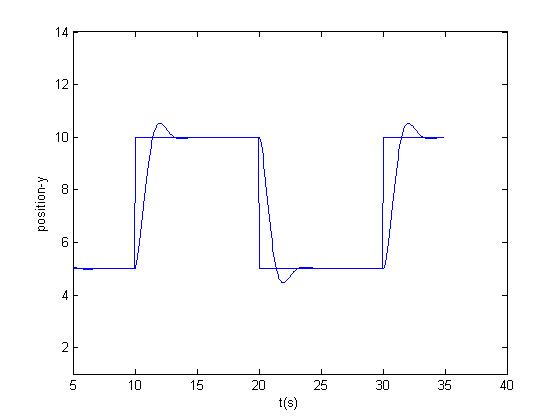
\includegraphics[width=\linewidth]{fig/gain8d1.jpg}
  \caption{kgain 8 and derivative 1}
\endminipage\hfill
\minipage{0.32\textwidth}%
  %\includegraphics[width=\linewidth]{shiva444.eps}
  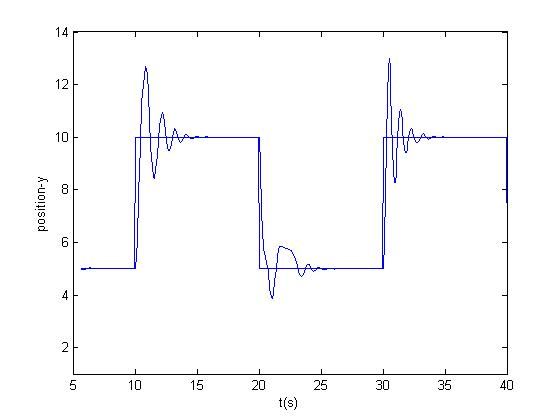
\includegraphics[width=\linewidth]{fig/gain100d1.jpg}
  \caption{kgain 100 and derivative 1}
\endminipage
\end{figure}
I tested 20 trials to find the best kgain. And I found out that for the derivative of 1, the best gain value is 4.

\begin{itemize}
\item different gain derivatives. I tested with the gain value of 4:
\end{itemize}

\begin{figure}[!htb]
\captionsetup{justification=centering}
\minipage{0.32\textwidth}
  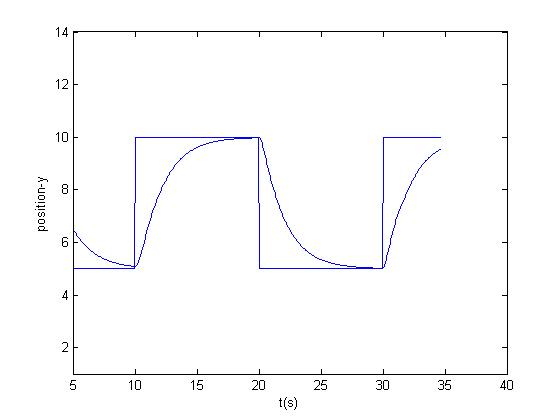
\includegraphics[width=\linewidth]{fig/gain4d2.jpg}
  \caption{kgain 4 and derivative 2}
\endminipage\hfill
\minipage{0.32\textwidth}
  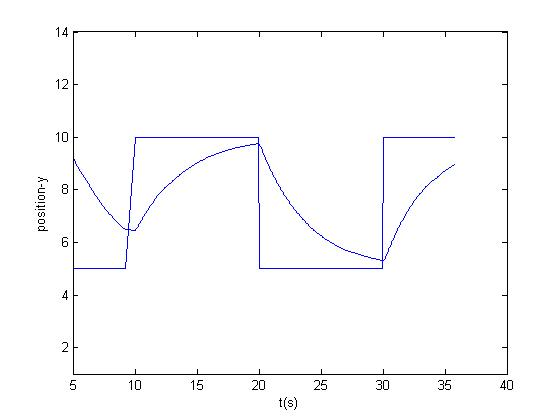
\includegraphics[width=\linewidth]{fig/gain4d4.jpg}
  \caption{kgain 4 and derivative 4}
\endminipage\hfill
\minipage{0.32\textwidth}%
  %\includegraphics[width=\linewidth]{shiva444.eps}
  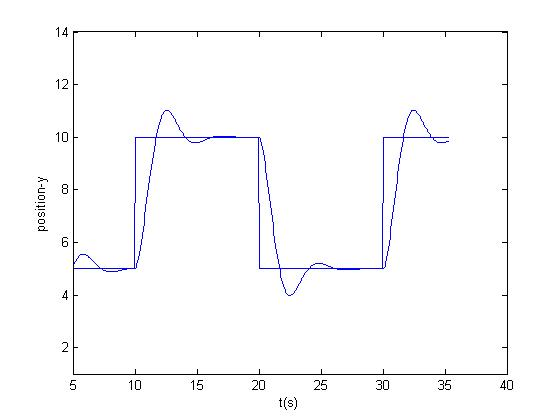
\includegraphics[width=\linewidth]{fig/gain4d05.jpg}
  \caption{kgain 4 and derivative 0.5}
\endminipage
\end{figure}
It shows that for the gain value 4, the best derivative is 1.
\begin{itemize}
\item Varying Brownian Noise:

For this purpose, I doubled Brownian gain and ran the code and waited a long time to see what happens gradually:
\begin{figure}[!htb]
\captionsetup{justification=centering}
\minipage{0.32\textwidth}
  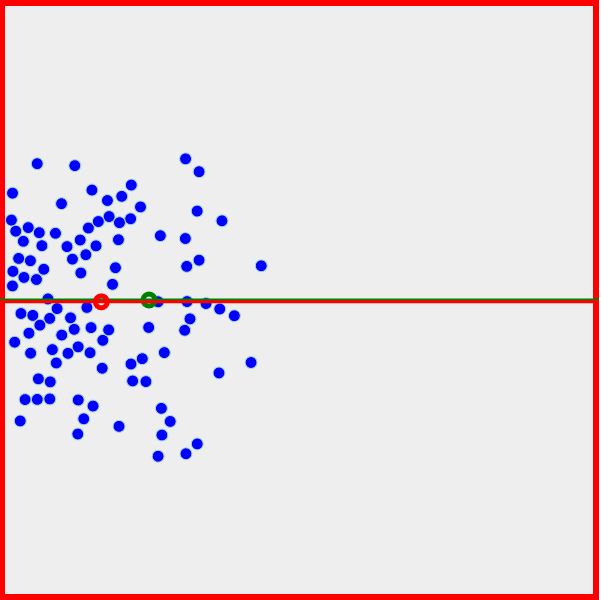
\includegraphics[width=\linewidth]{fig/brownian2in11.png}
  \caption{Brownian Effect after 11 seconds}
\endminipage\hfill
\minipage{0.32\textwidth}
  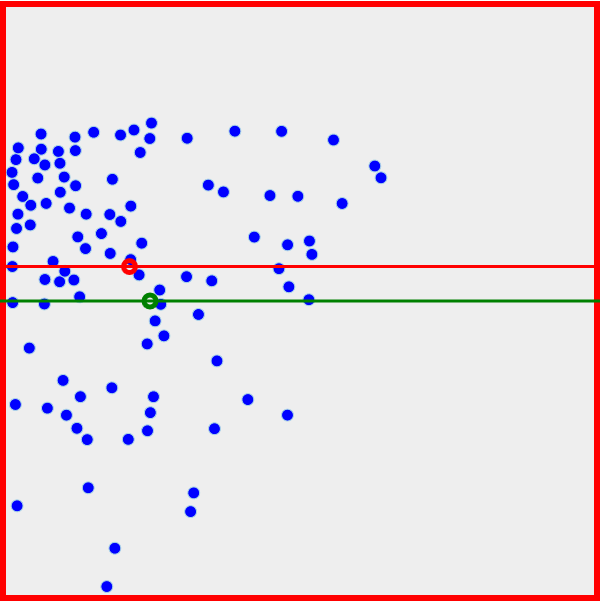
\includegraphics[width=\linewidth]{fig/brownian2in45.png}
  \caption{Brownian Effect after 45 seconds}
\endminipage\hfill
\minipage{0.32\textwidth}%
  %\includegraphics[width=\linewidth]{shiva444.eps}
  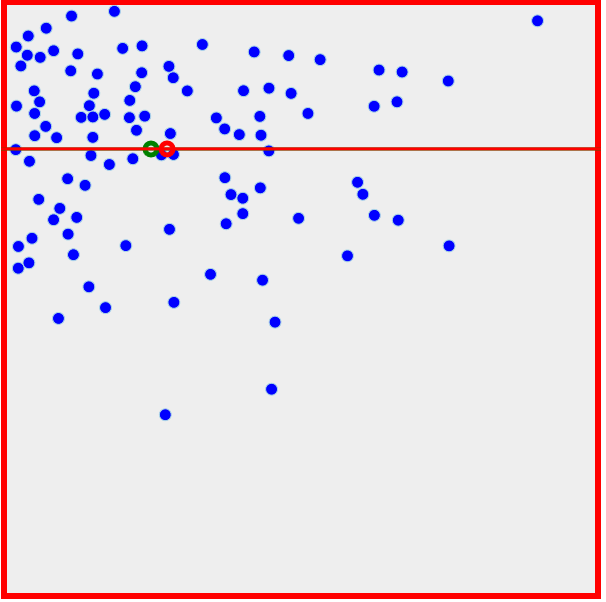
\includegraphics[width=\linewidth]{fig/brownian2in86.png}
  \caption{Brownian Effect after 86 seconds}
\endminipage
\end{figure}
As we can see in the images, the mean position of the \emph{x} axis will go to the center of the line gradually. After infinity we have the following image:
\begin{figure}[h]
\begin{center}
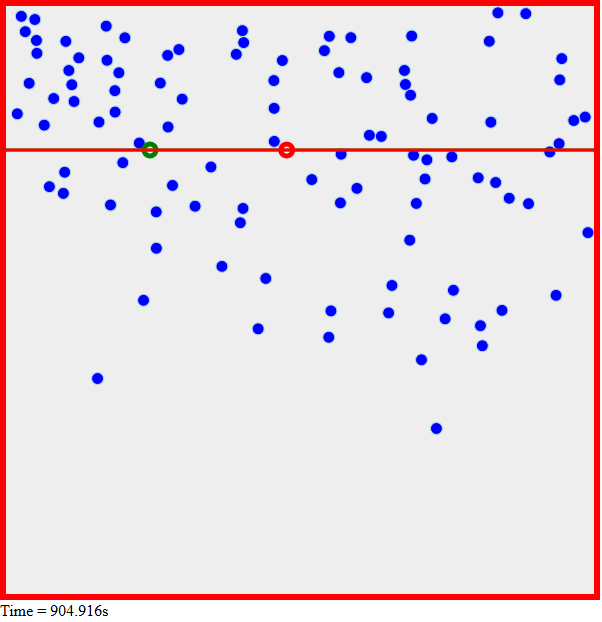
\includegraphics[width=5cm]{fig/brownian2infinity.png}
\caption{As t goes to infinity}
\end{center}
\end{figure}

which means that if we don't control it, it will spread completely.

\item 2D control
Now we can control mean of \emph{x} too:
\begin{figure}[!htb]
\captionsetup{justification=centering}
\minipage{0.32\textwidth}
  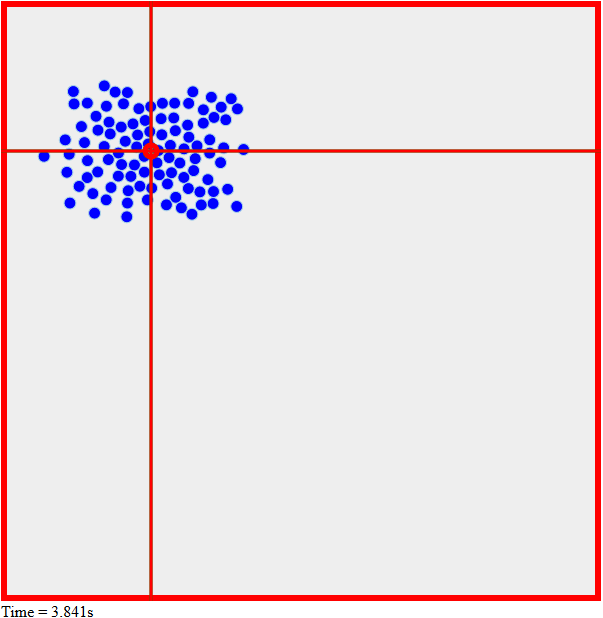
\includegraphics[width=\linewidth]{fig/2DControl3.png}
  \caption{The goal position is 5 and 5}
\endminipage\hfill
\minipage{0.32\textwidth}
  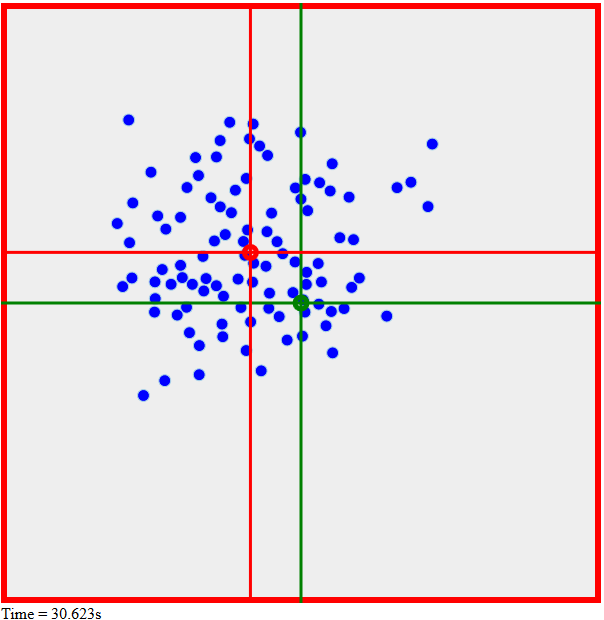
\includegraphics[width=\linewidth]{fig/2DControl2.png}
  \caption{Going to the goal position}
\endminipage\hfill
\minipage{0.32\textwidth}%
  %\includegraphics[width=\linewidth]{shiva444.eps}
  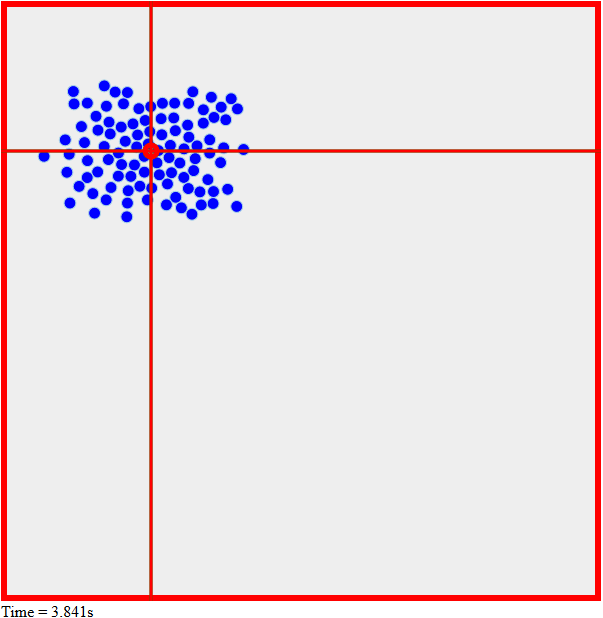
\includegraphics[width=\linewidth]{fig/2DControl3.png}
  \caption{The goal position is 10 and 10}
\endminipage
\end{figure}
\end{itemize}

\section{My \emph{Plan} for next week}

\begin{itemize}
\item Applying variance and covariance and standard deviation. 
\item Which one of them is the best?
\end{itemize}

\subsection{Meeting with Dr. Becker On Wednesday 19th, 1 pm }

\begin{itemize}
\item Deciding what to take for the next semester
\item What to survey for lab access
\item Show him results.
\end{itemize}

\end{document}
